In this chapter I explain my preparatory work, which mainly consists of understanding the problem from the mathematical and research point of view.
First, I explain in detail why measuring robustness of graph metrics is an important and a novel field, describing in detail the work done in ``The Paper'' that this dissertation is based on.
Further I introduce specific definitions of graph metrics and robustness measures that I use in the implementation.


\section{Introduction to confidence}

Statistical significance, confidence scores, confidence intervals, error ranges, all are used to signal or approximate the extent to which the observed result is reliable.
Some of the confidence values are a direct probability that an error is made, given the available evidence, such as a statistical significance when rejecting a null hypothesis, or confidence intervals.
Other error values such as error ranges or standard deviations estimate how much off a numerical value may be.
These error measures are all important to state and assess how precise or confident an experiment or an observation is.

A research result without assessing its precision or confidence can be considered incomplete.
We need the assessment of possible error to derive any further guidance from the research.\citeneeded

However, can we measure the precision, or the confidence or graph metrics?
If research is based on evaluating metrics on graphs which are themselves imprecise or having possible errors in the structure, how can we assess the confidence or precision of such result?


\section{The Paper}

This dissertation project is based on, and extending the ideas from the paper by Bozhilova et al.: \textsl{Measuring rank robustness in scored protein interaction networks}\cite{Bozhilova2019}.
From now on, I will refer to it as \textsl{The Paper}.

\subsection{Protein networks}

Protein networks is a large research field with a plethora of uses, and investigating them is important for the future of bioinformatics~\todo{examples + citations}.

Most graph datasets obtained from the real-world, including protein interaction networks (PINs), are a result of experiments or observations which possibly introduce measurement errors, either systematic or random errors.

Also, protein networks have a specific structure: nodes represent proteins and weighted (or scored) edges represent the presence of interactions between proteins.
It is assumed that such interactions are mutual, therefore the formed graph is undirected.

\begin{figure}[ht]
    \vspace*{-3mm}
    \tikzset{every picture/.style={line width=0.75pt}} %set default line width to 0.75pt
    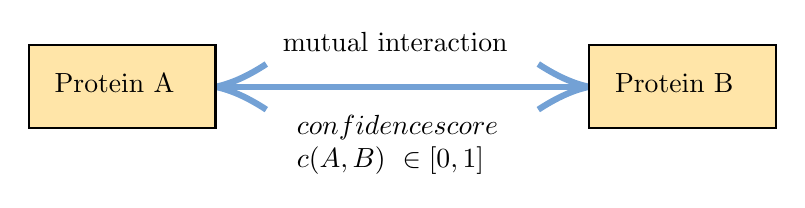
\begin{tikzpicture}[x=0.75pt,y=0.75pt,yscale=-1,xscale=1]
        %uncomment if require: \path (0,136); %set diagram left start at 0, and has height of 136

        %Straight Lines [id:da5202946805882411]
        \draw [color={rgb, 255:red, 115; green, 161; blue, 213 }  ,draw opacity=1 ][fill={rgb, 255:red, 0; green, 0; blue, 0 }  ,fill opacity=1 ][line width=2.25]    (114,40) -- (286,40) ;
        \draw [shift={(290,40)}, rotate = 180] [color={rgb, 255:red, 115; green, 161; blue, 213 }  ,draw opacity=1 ][line width=2.25]    (24.48,-10.98) .. controls (15.57,-5.15) and (7.41,-1.49) .. (0,0) .. controls (7.41,1.49) and (15.57,5.15) .. (24.48,10.98)   ;
        \draw [shift={(110,40)}, rotate = 0] [color={rgb, 255:red, 115; green, 161; blue, 213 }  ,draw opacity=1 ][line width=2.25]    (24.48,-10.98) .. controls (15.57,-5.15) and (7.41,-1.49) .. (0,0) .. controls (7.41,1.49) and (15.57,5.15) .. (24.48,10.98)   ;
        %Shape: Rectangle [id:dp8315683426496481]
        \draw  [fill={rgb, 255:red, 255; green, 229; blue, 168 }  ,fill opacity=1 ] (20,20) -- (110,20) -- (110,60) -- (20,60) -- cycle ;
        %Shape: Rectangle [id:dp6227729030936355]
        \draw  [fill={rgb, 255:red, 255; green, 229; blue, 168 }  ,fill opacity=1 ] (290,20) -- (380,20) -- (380,60) -- (290,60) -- cycle ;

        % Text Node
        \draw (31,32) node [anchor=north west][inner sep=0.75pt]   [align=left] {Protein A};
        % Text Node
        \draw (301,32) node [anchor=north west][inner sep=0.75pt]   [align=left] {Protein B};
        % Text Node
        \draw (141,12) node [anchor=north west][inner sep=0.75pt]   [align=left] {mutual interaction};
        % Text Node
        \draw (141,50.4) node [anchor=north west][inner sep=0.75pt]    {$ \begin{array}{l}
                                                                              \text{confidence score}\\
                                                                              c( A,B) \ \in [ 0,1]
        \end{array}$};
    \end{tikzpicture}
    \caption{Schematic of an interaction between two proteins}
    \vspace*{-2mm}
\end{figure}


\subsection{Confidence scores}

The weight of each edge represents a confidence score which may be a value, or a set of values, describing some sort of \textsl{likelihood} that the given interaction is true, given the available evidence.
They do \textsl{not} indicate the strength or intensity of the interaction (which would be a different property, usually not observed in such protein networks).

For example, in the STRING database of protein networks used in The Paper, the main interaction score is an approximated \textsl{confidence} based on evidence such as scientific experiments, genetic observations (gene fusions, gene co-occurrence), statistical predictions, text mining of scientific articles, or existing knowledge (other available protein interaction databases)~\cite{Szklarczyk2019}.
The database then contains score values for each type of evidence, as well as a combined overall confidence score.
The Paper, as well as my dissertation, use only the combined confidence score and do not focus on the biological details of each evidence type.

\begin{figure}
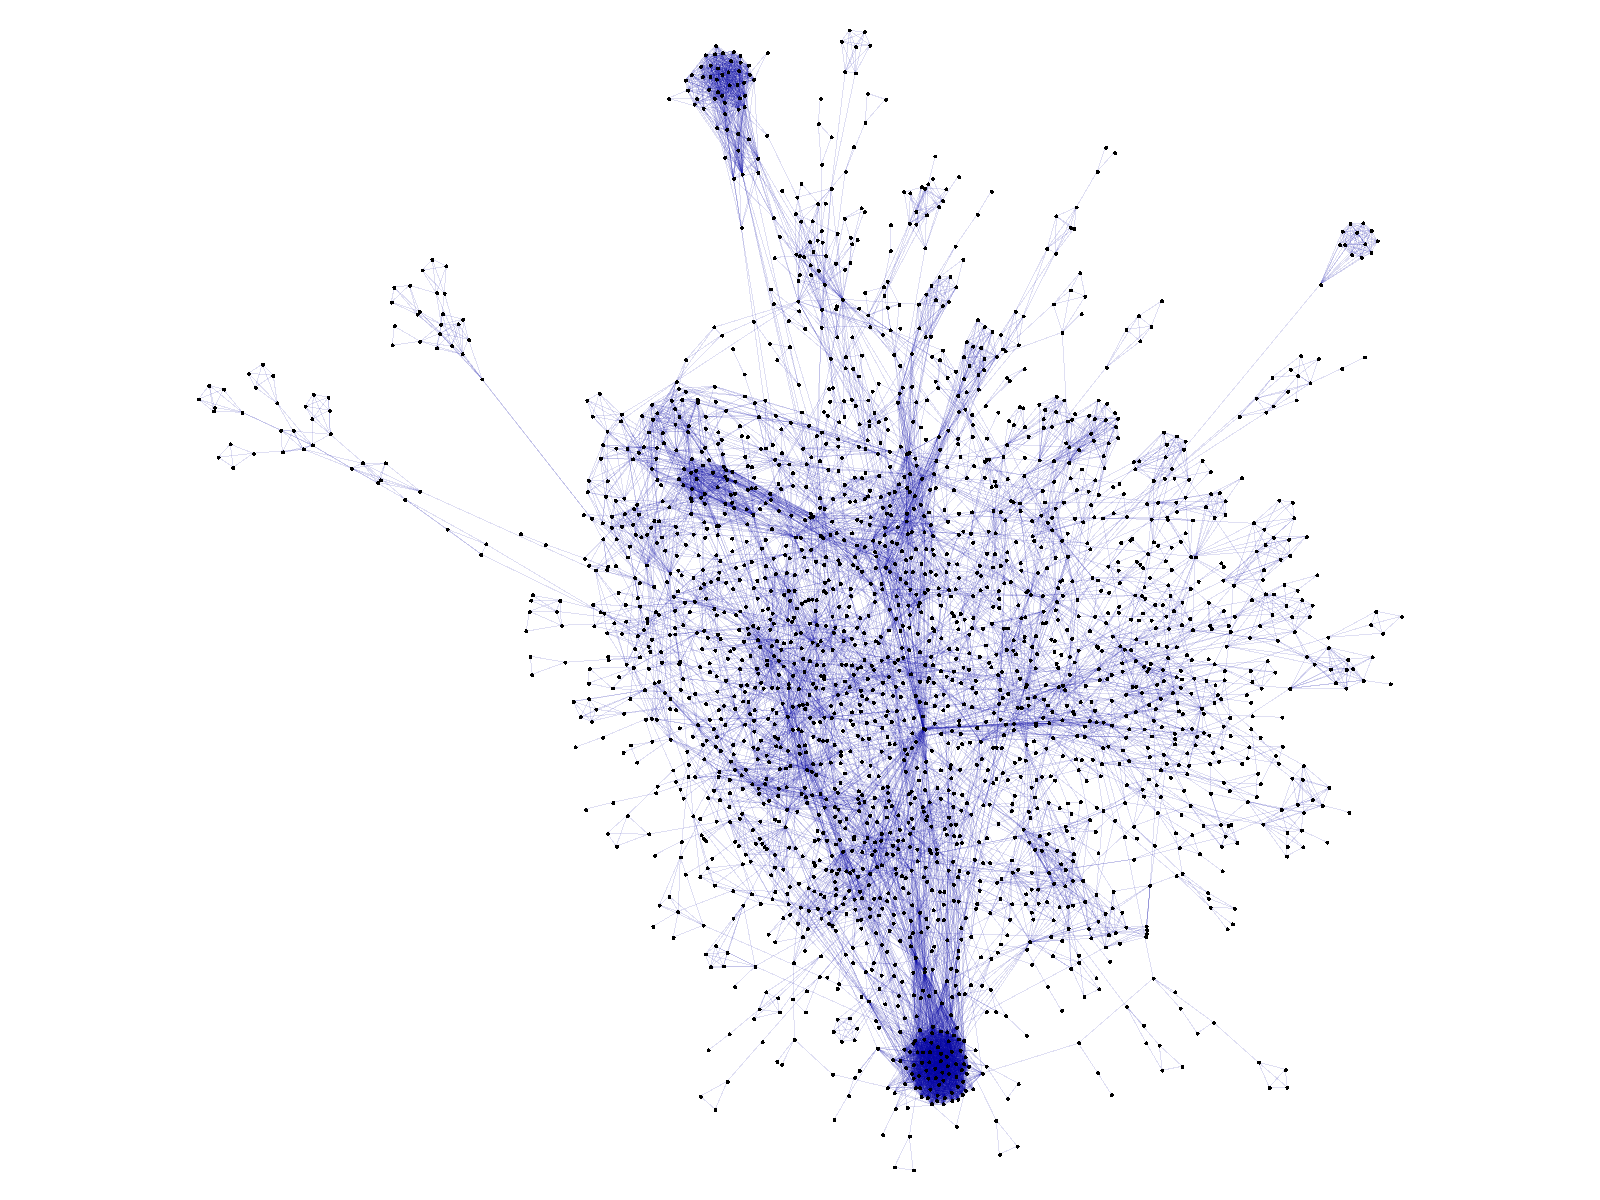
\includegraphics[height=8cm]{ecoli_giant_at_900.png}
\caption{An interaction network of proteins from the \textit{Escherichia coli} organism from the STRING database, thresholded at the $0.9$ score (high confidence). Only nodes of the giant component are shown.}
\label{fig:ecoli_giant_at_900}
\end{figure}


When researching protein interactions, in practice, researchers choose a \textbf{threshold} and then form a protein interaction network from the database considering only interactions (edges) whose confidence score is greater than the selected threshold, to only take into account interactions of sufficiently high quality.
Researchers then use tools such as graph metrics to identify important nodes or components of graphs, calculate statistics, or derive other results.

\autoref{fig:ecoli_giant_at_900} shows an example of a protein network taken from the STRING database\cite{Szklarczyk2019}, of proteins of the \textit{Escherichia coli} organism.
Only edges with score of $0.9$ corresponding to the ``highest confidence'' level (on the scale from $0$ to $1$) were retained, and only the giant connected component of it is shown.
That yields a graph with 2382 nodes and 12071 edges.

\subsection{Metric robustness}

However, as The Paper remarks, the analysis based on metric evaluation can be sensitive to the choice of the threshold.
If a node metric is to be useful for extracting biological signal, it should lead to similar results across networks obtained at different reasonable confidence score thresholds.
Hence, the point of studying metric robustness or \textsl{stability} is a way to assess how reliable the results are on a graph derived from a given threshold.

It is clear that numerical values of node metrics will depend on such threshold, for example the degree and the clustering coefficient of each node will indeed monotonically decline with declining density of the network, which monotonically declines as we increase the confidence threshold.
For this reason, the point of The Paper is to assess a robustness of graph metrics based on the \textbf{rankings} of nodes induced by each metric (where ranking is just a total preorder of the nodes based on the metric values).

\subsubsection{Rank robustness}

The Paper introduces three different measures assessing robustness of node metrics (all will be explained later):
\begin{itemize}
    \item rank continuity,
    \item rank identifiability,
    \item rank instability.
\end{itemize}
All three measures are based on rankings of nodes induced by node metrics, and not on the exact values, to mitigate the density bias described above.

The Paper studies robustness of 25 different \textsl{node} metrics only, i.e. graph metrics which return one numerical value per node.


\section{Mathematical background}

In this section I review background material on graph theory and examining graph metric robustness, and fix terms I will use later to avoid ambiguity in further chapters.

In particular, this section will focus introducing high-level concepts of:
\begin{itemize}
    \item relevant bits of graph theory
    \item graph metrics
    \item ranking
    \item metric robustness
\end{itemize}

\subsection{Graphs}

Graphs (or networks) from graph theory usually consist of \textit{components} (or nodes, vertices) and \textit{links} between them (edges).
Some definitions in this subsection are based on the book \textsl{A first course in network theory}\cite{Estrada2017}.

\begin{definition}[Graph]
    Let $V$ be a finite set of $n$ nodes (or vertices), and let $E \subseteq V \times V$ be a set of edges.\\
    A \textbf{graph} $G$ is a pair $(V, E)$.\\
    $V$ is the \textbf{node set} of $G$, and $E$ is the \textbf{edge set} of $G$.
\end{definition}

Real-world data (or datasets) in the form of graphs are also called \textbf{networks}.
Still, I may interchange the words \textsl{graph}, \textsl{network} and \textsl{dataset}, but generally:
\begin{itemize}
    \item \textsl{dataset} is data stored in its raw form, such as a file downloaded from the Internet
    \item \textsl{network} is the real-world graph-like data conveyed by a dataset
    \item \textsl{graph} is a hypothetical structure, also a mathematical interface or representation that algorithms work with
\end{itemize}

\begin{definition}[Graph properties]
    \begin{itemize}[leftmargin=*]
        \item $G$ is \textbf{reflexive} iff $\forall v \in V.\ (v, v) \in E$
        \item $G$ is \textbf{anti-reflexive} iff $\forall v \in V.\ (v, v) \notin E$
        \item $G$ is \textbf{undirected} (or equally \textbf{symmetric}) iff $\forall v_1, v_2 \in V.\ (v_1, v_2) \in E \Leftrightarrow (v_2, v_1) \in E$
        \item $G$ is \textbf{directed} iff it is not undirected
        \item $G$ is a \textbf{simple graph} iff it is undirected and anti-reflexive
    \end{itemize}
\end{definition}

Graphs I use in this project are all \textsl{simple graphs} (unless stated otherwise), i.e. edges are undirected (or bi-directional), and always span two different nodes.

\begin{wrapfigure}[11]{R}{0.31\textwidth}
\vspace*{-10mm}
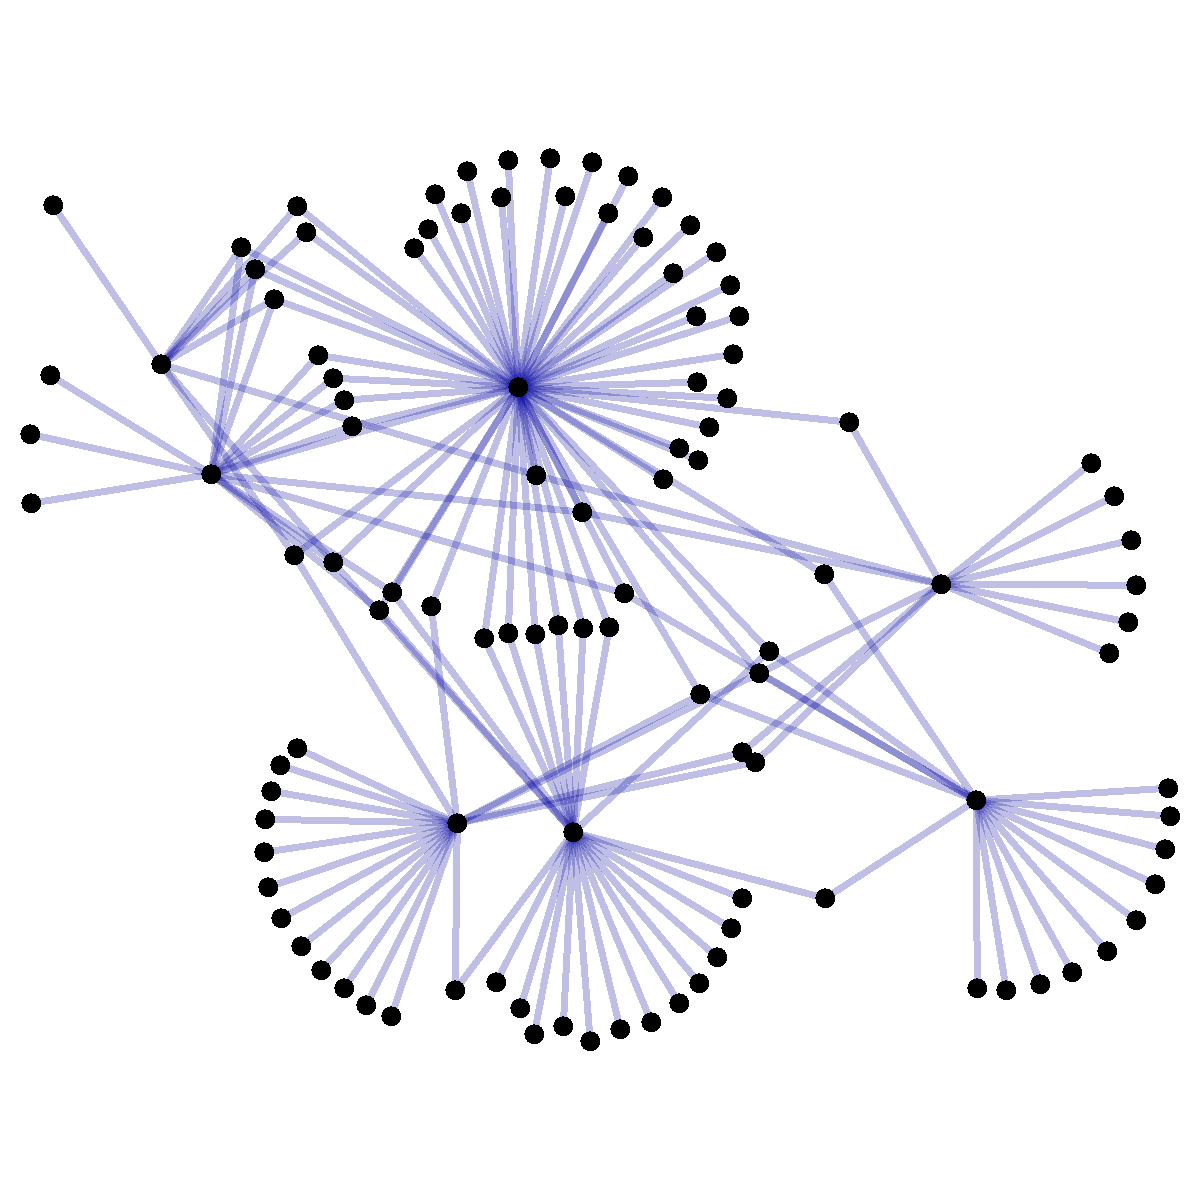
\includegraphics[width=\linewidth]{simple_graph.png}
\vspace*{-10mm}
\caption{A small example of a \textsl{connected} \textsl{simple} graph (\textsl{undirected} and \textsl{anti-reflexive}).}
\label{fig:simple_graph}
\end{wrapfigure}


\autoref{fig:simple_graph} is an illustration of a connected simple graph with 110 nodes and 151 edges.
I used graphs like this for testing purposes when developing \graffs.

\begin{definition}[Relations on graphs]
    \begin{itemize}[leftmargin=*]
        \item $G' = (V', E')$ is a \textbf{subgraph} of $G = (V, E)$ iff $V' \subseteq V$ and $E' \subseteq E$
        \item Let $G_1 = (V_1, E_1)$ and $G_2 = (v_2, E_2)$, then $G_1 \cup G_2 = (V_1 \cup V_2, E_1 \cup E_2)$ is the \textbf{union} of the two graphs, and $G_1 \cap G_2 = (V_1 {\cap} V_2, E_1 {\cap} E_2)$ is the \textbf{intersection} of the two graphs.
    \end{itemize}
\end{definition}

\begin{definition}[Node adjacency]
    \begin{itemize}[leftmargin=*]
        \item In an undirected graph, $v_1$ is \textbf{adjacent} to $v_2$ iff $(v_1, v_2) \in E$
        \item A \textbf{loop} is an edge of the form $(v, v)$.
        Note that simple graphs have no loops.
        \item Define $\deg^-(v) = \left| \Set{v' \in V}{(v', v) \in E} \right|$ to be the \textbf{indegree} of $v$, and $\deg^+(v) = \left| \Set{v' \in V}{(v, v') \in E} \right|$ to be the \textbf{outdegree} of $v$, in other words, the number of incoming and outcoming edges, respectively.
        If the graph is undirected, then $\deg^-(v) = \deg^+(v) = \deg(v)$ is called \textbf{degree}.
        \item For $G = (V, E)$ with $V = {1, 2, \dots, n}$, define $A = (a_{ij})$ to be the \textbf{adjacency matrix} of $G$ where
        \[ a_{ij} = \begin{cases}
                        1, & \textnormal{if}\ (i, j) \in E \\
                        0, & \textnormal{if}\ (i, j) \notin E
        \end{cases} \]
        for $1 \leq i, j \leq n$.

        Note that adjacency matrix of undirected graph is symmetric.
    \end{itemize}
\end{definition}

\begin{definition}[Connectedness]
    \begin{itemize}[leftmargin=*]
        \item $u, v$ are \textbf{connected nodes} is there exists a path between $u, v$ in $G$, i.e. if $(A^k)_{uv} = 1$ for some $k\in \mathbb{N}$.
        \item $G = (V, E)$ is \textbf{connected graph} if $\forall v_1, v_2 \in V. v_1, v_2$ are connected nodes.
        \item A subgraph $G' \subseteq G$ is a \textbf{(connected) component} iff $G'$ is a maximal connected subgraph of $G$.

        Note that all components of a graph are disjoint, therefore each node belongs to exactly one component.
    \end{itemize}

    \item A \textbf{giant component} of a graph is a single component that has more nodes than any other component of the graph.

    Note that a giant component may not exist, if more components have maximum number of nodes.
\end{definition}

\begin{figure}
\vspace*{-4mm}
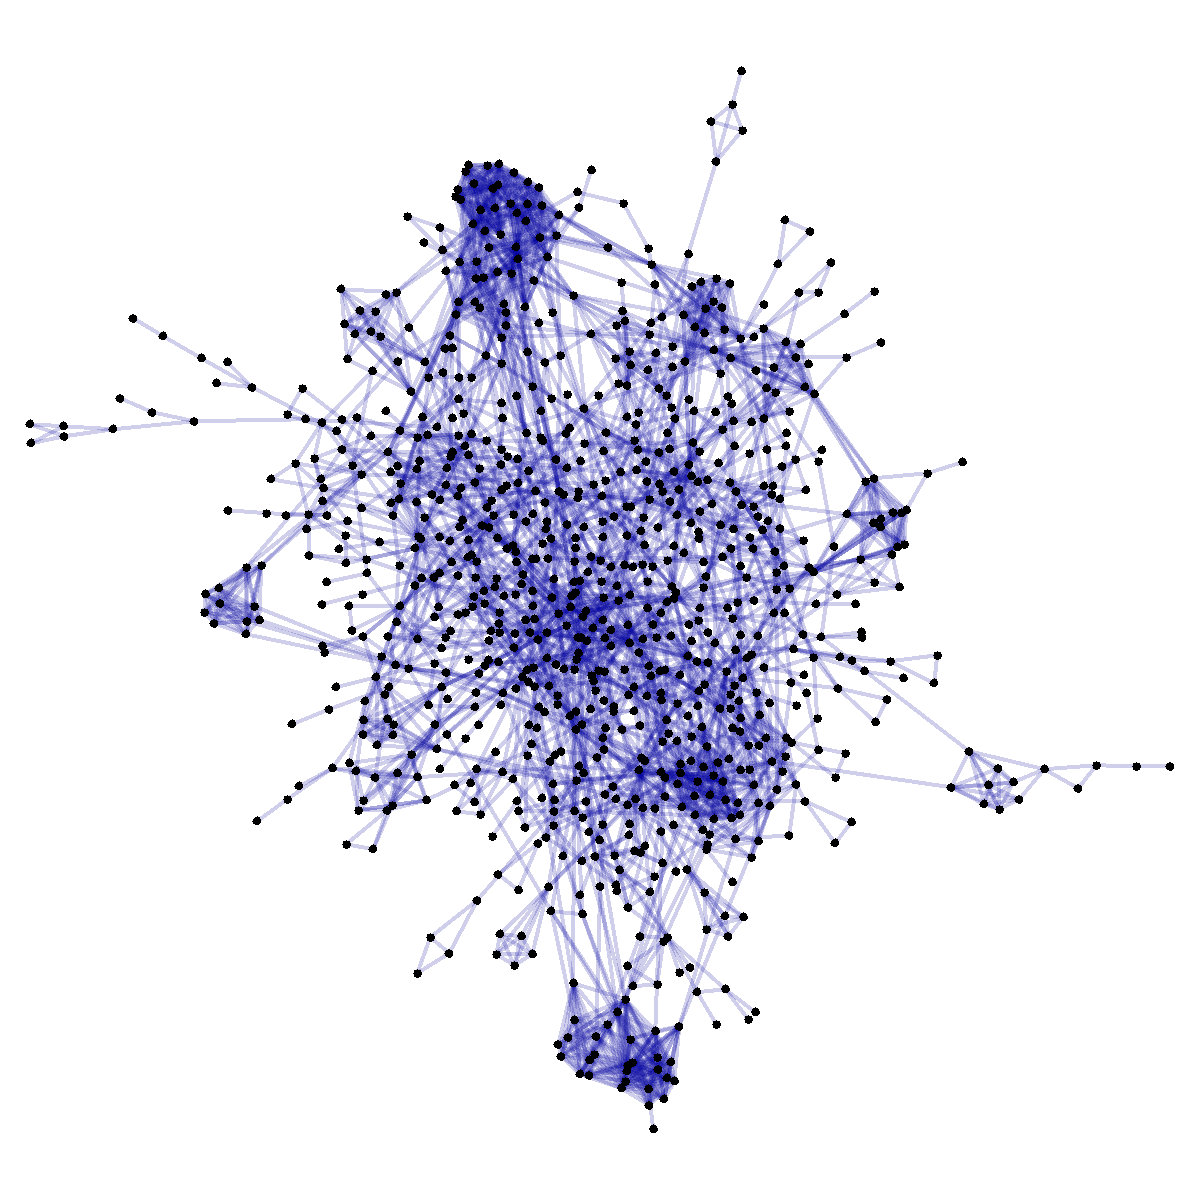
\includegraphics[height=6cm]{disconnecting_graph.png}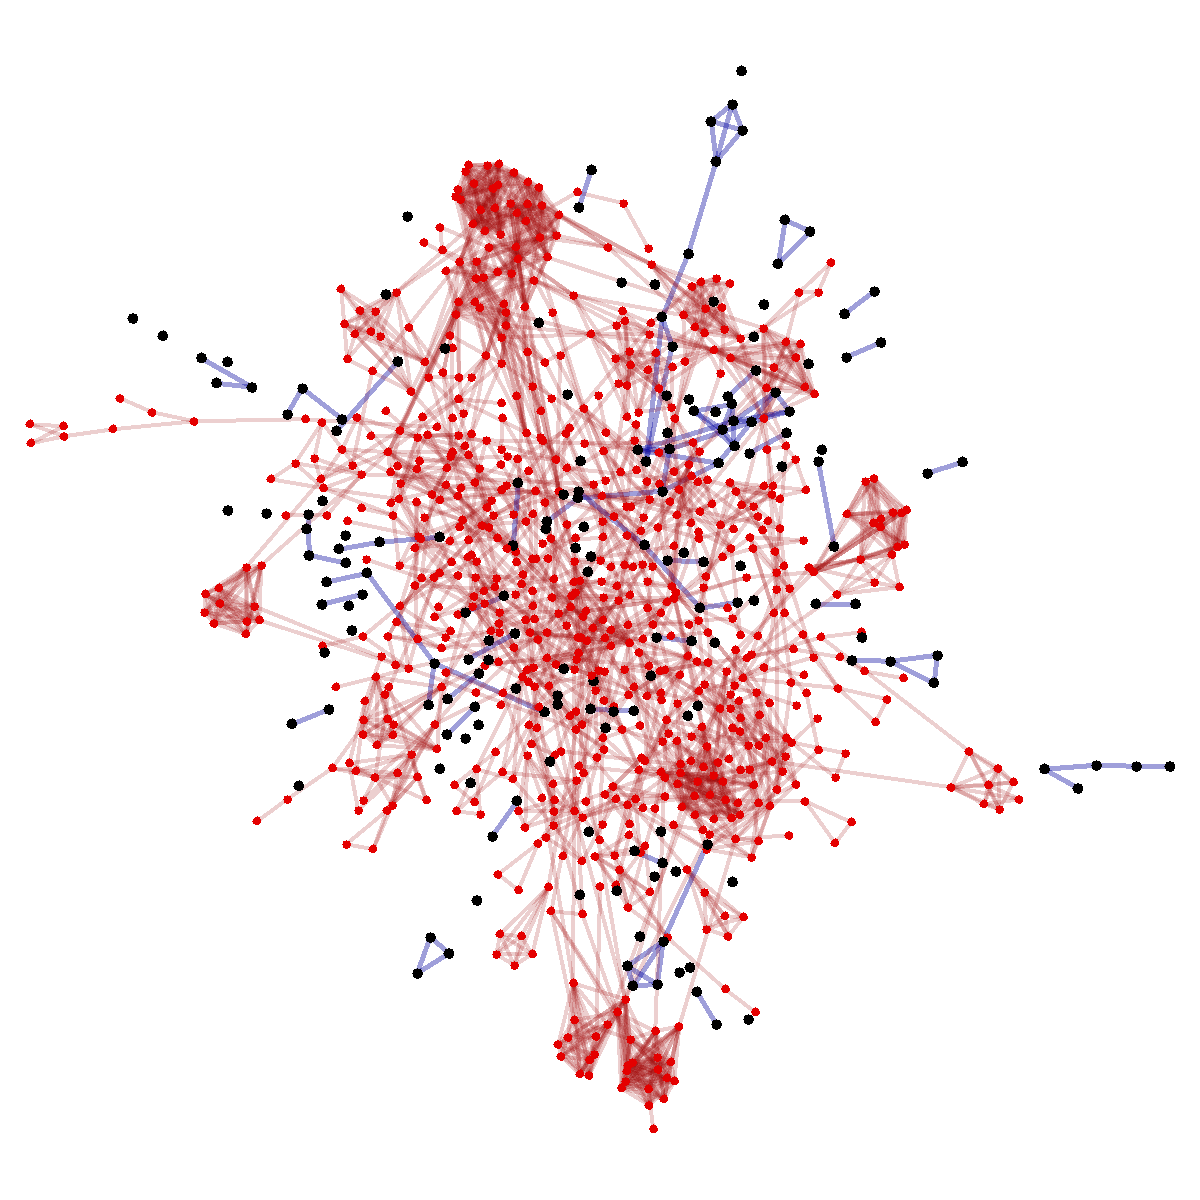
\includegraphics[height=6cm]{disconnecting_graph2.png}
\vspace*{-4mm}
\caption{Illustrated is how thresholding (a subgraph of) a protein network (left) results in one giant component (red) and multiple small disconnected components.
The left is a certain subgraph of the \textit{ecoli} dataset (all edges with confidence $>0.4$), the right graph has only edges with confidence $>0.5$.}
\label{fig:disconnecting_graph}
\end{figure}


Most of real-world networks (such as social networks, citation networks and even protein interaction networks) contain a single giant component, and some small isolated components.
For example, in \autoref{fig:disconnecting_graph}, the red nodes form a giant component of the graph.


%\subsubsection{Networks}
%
%Moving towards real-world data, graphs often emerge from a certain source in the world.
%Just a few examples of the data possibly represented by graphs include social networks, road networks, computer networks, protein interaction networks, citation networks, web networks and so on.
%In this work I distinguish graphs and networks, although I may sometimes interchange these two.
%
%\begin{definition}[Network]
%    A \textbf{network} is a graph whose nodes or edges can have attributes $\textnormal{attr}_v, \textnormal{attr}_e : \Sigma^* \rightarrow \mathbb{U}$ for some set of possible identifiers $\Sigma^*$ (such as a language over an alphabet $\Sigma$) and a value domain $\mathbb{U}$ (such as $\mathbb{R}$ or $\mathbb{R}^2$)
%\end{definition}
%
%Graphs and networks allow capturing the same structure, however, the main difference is that nodes of a network are \textit{identifiable}, while we rarely consider \textit{identity} of graph nodes.
%%This is because nodes and edges of graphs coming from real-world are often (nearly) isomorphic to real-world objects and relations between them.
%There may be either an exact or inexact matching between nodes/edges in the graph and objects/relations in the real world where the data came from (depending on whether the dataset is an approximation of the world).
%I will often use networks when describing knowledge of the world.
%
%\begin{definition}[Graph matching]
%    Given two graphs $G = (V, E)$ and $G' = (V', E')$ derived from the same network, define \textbf{graph matching}, $M$, to be a bijection $V \leftrightarrow V'$ such that $(v, v') \in M$ iff $v, v'$ correspond to, or come from the same node in the network.
%\end{definition}
%
%For measuring metric robustness it will be beneficial to know matching between multiple graphs coming from the same dataset, or in other words to preserve identity of nodes across such graphs.

\subsection{Graph metrics}

Metrics are essentially functions of graphs that assign a value to each node.
Metrics are used to quantify various properties of graphs, identifying important nodes in different contexts, describing graph structures, comparing different graphs and more.
I study graph metrics as they are prominent and becoming even more crucial in analysing graphs of ever-growing real-world data.

In this section I describe some of the metrics that are most significant for analysing protein interaction networks, and other graphs used in this project.
The set of these metrics and their specific definition is based on The Paper\cite{Bozhilova2019}, and on~\cite{MartinHernandez2011}.

The metrics below are defined for \textsl{undirected} graphs.

\subsubsection{Degree}

One of the simplest metrics calculates the degree of each node.

\begin{definition}[Degree (centrality)]
    For a graph $G = (V, E)$, define \textbf{degree centrality} $DC : V \rightarrow \mathbb{N}$ to be
    \[ DC(v) \eqdef \deg(v) = \left| \Set{v' \in V}{(v', v) \in E} \right| \]
\end{definition}

\subsubsection{Closeness centrality}

Closeness centrality of a node $v$ is the reciprocal value of the sum of $d(v, i)$, the distances from that node to all other nodes $i$ in the graph.

\begin{definition}[Closeness centrality]
    \[CC(v) = \frac{1}{\sum_{i \neq v} d(v, i)}\]
\end{definition}

This is well-defined for connected graphs, however, $d(v, i)$ is undefined if $v, i$ belong to two different components of the graph.
For disconnected graphs, I set $d(v, i) = |V|$ to follow the approach in The Paper.

Closeness centrality measures the reciprocal of the \textsl{farness} of each node to other nodes.
Nodes with higher closeness centrality are \textsl{closer} to all other nodes.

A common alternative for disconnected graphs is to compute Harmonic centrality.

\begin{figure}
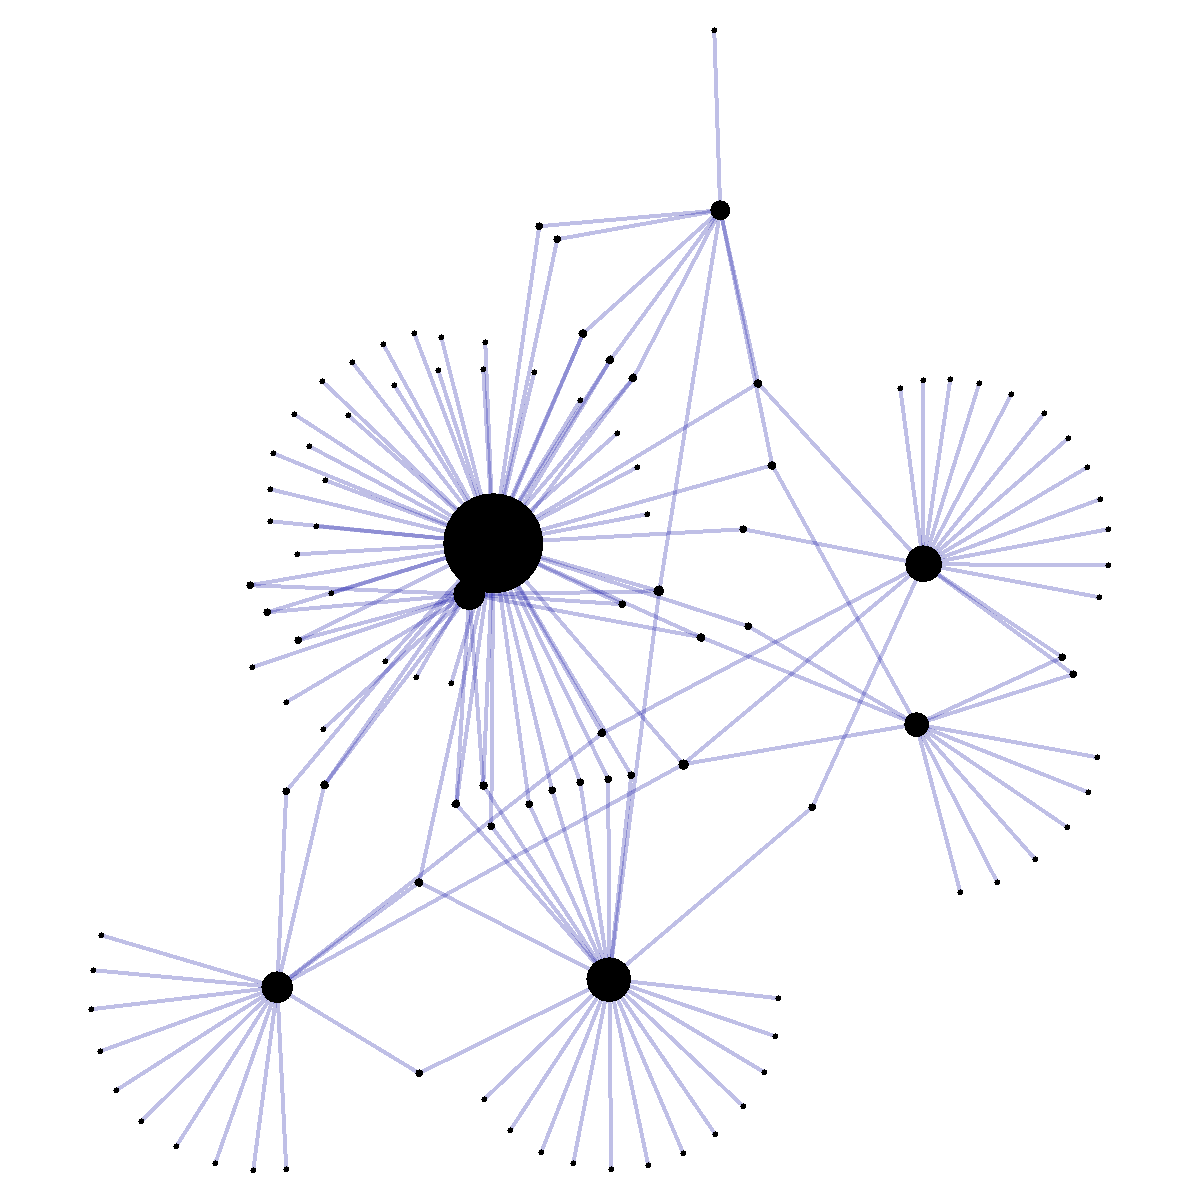
\includegraphics[height=5cm]{simplegraph_by_some_metrics.png}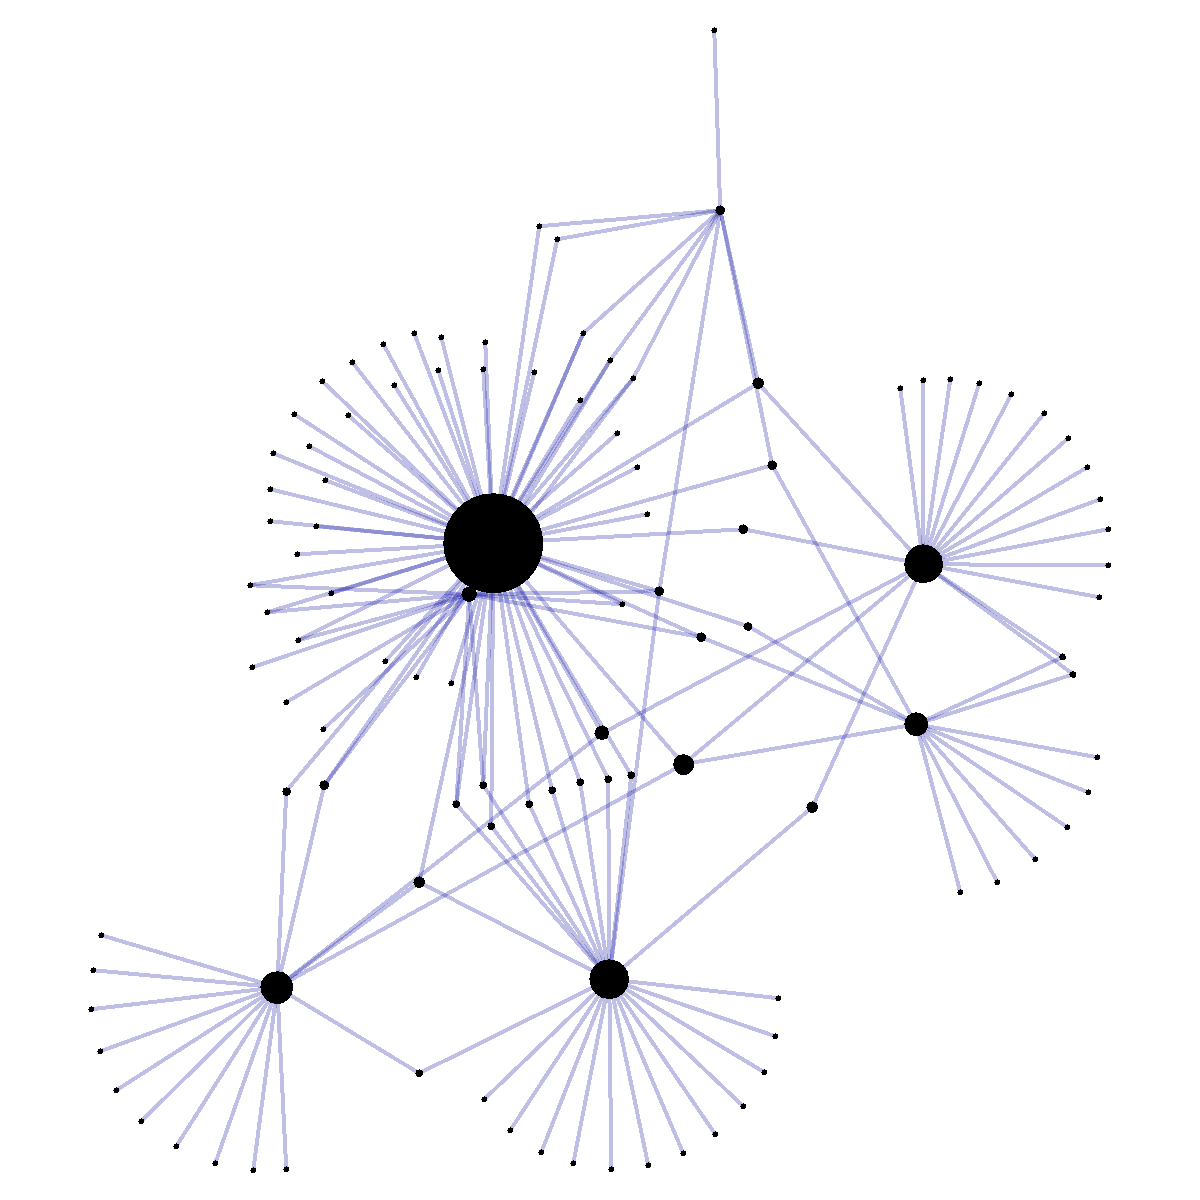
\includegraphics[height=5cm]{simplegraph_by_some_metrics2.png}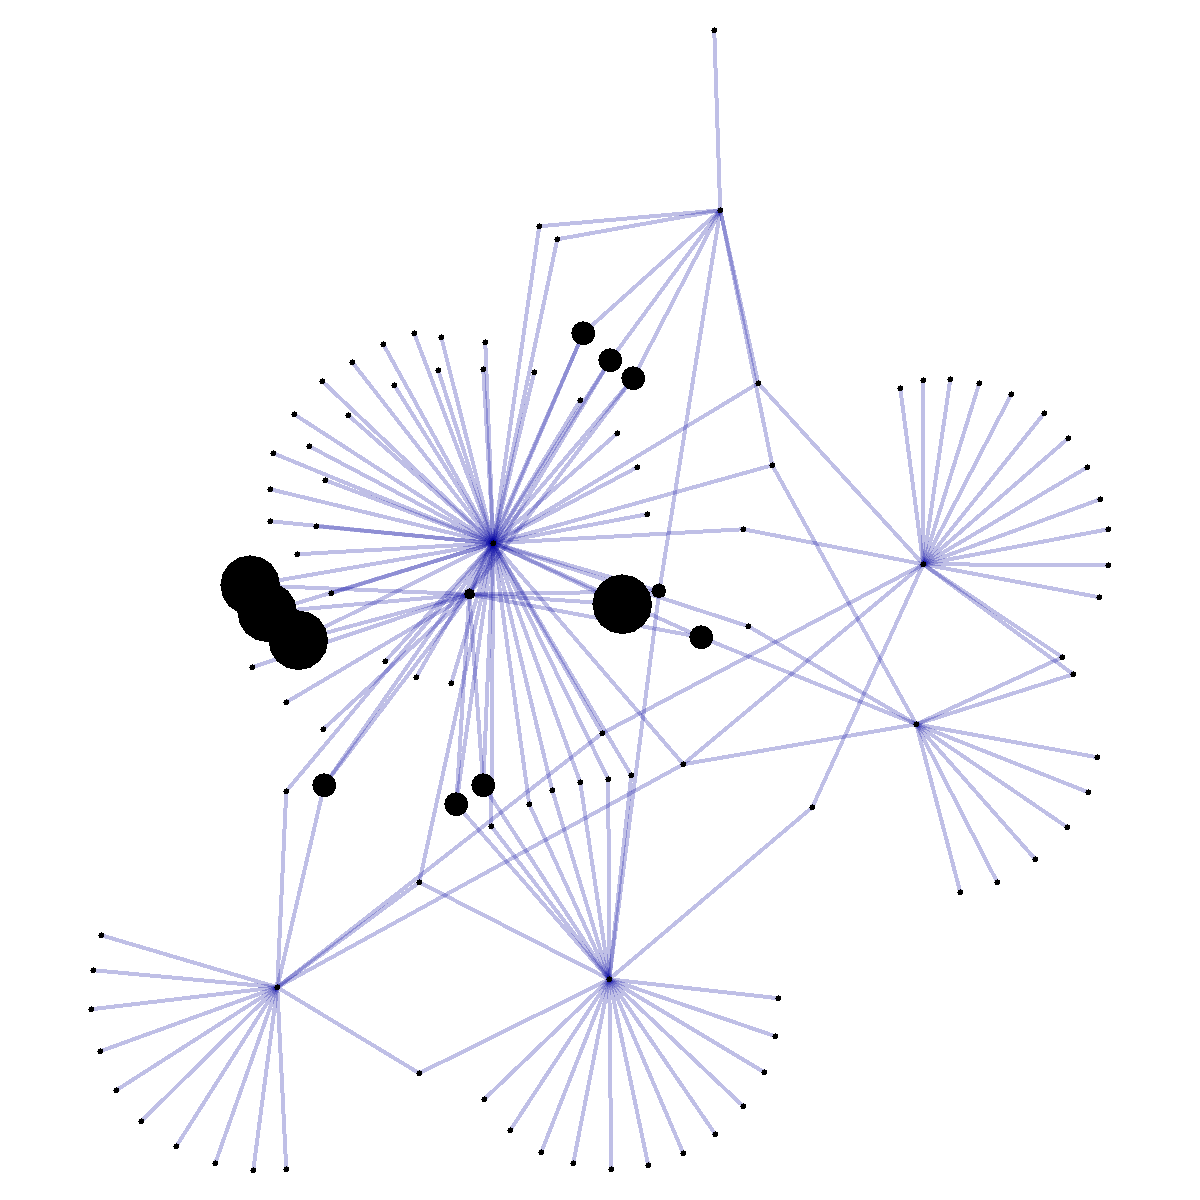
\includegraphics[height=5cm]{simplegraph_by_some_metrics3.png}
\caption{A simple graph with each node's diameter proportional to its \textsl{degree} (1), \textsl{betweenness centrality} (2), and \textsl{local clustering} (3).
In this particular graph, (1) and (2) show similar characteristics (greater value for more ``central'' nodes), whereas local clustering is significantly different.}
\label{fig:simplegraph_by_some_metrics}
\end{figure}


\subsubsection{Harmonic centrality}

Has similar meaning to closeness centrality, and a similar definition.

\begin{definition}[Harmonic centrality]
    \[HC(v) = \sum_{i \neq v} \frac{1}{d(v, i)}\]
    with $1 / d(v, i) = 0$ for disconnected nodes $v, i$.
\end{definition}

%\subsubsection{Eigenvector centrality}
%
%\subsubsection{Katz centrality}
%- not used much recently
%
%\subsubsection{PageRank}
%= Katz centrality, but divide each vertex's contribution by its out-degree
%
%\subsubsection{Hyperlink-induced topic search (HITS)}
%Hubs and authorities, by Kleinberg

% from GraphStream
%
%\subsubsection{CommunityMeasure}
%- Modularity\\
%- Community Distribution\\
%- CommunityRelativeMeasure $\rightarrow$ NormalizedMutualInformation $\rightarrow$ VariationOfInformation
%
%\subsubsection{Eccentricity}
%
%\subsubsection{Surprise measure}
%

\subsection{Ranking}

\begin{definition}[Preorder]
    Binary relation $\sqsubseteq$ on some set $P$ is a \textbf{preorder} iff it is reflexive and transitive, i.e.:
    \begin{itemize}
        \item $\forall a, b \in P.\ a \sqsubseteq a$ \tabto{7.3cm}(reflexivity)
        \item $\forall a, b, c \in P.\ (a \sqsubseteq b \wedge b \sqsubseteq c) \implies a \sqsubseteq c$ \tabto{7.3cm}(transitivity)
    \end{itemize}
\end{definition}

\begin{definition}[Total preorder]
    A binary relation $\sqsubseteq$ on some set $P$ is a \textbf{total preorder} iff it is a preorder and a connex relation, i.e.:
    \begin{itemize}
        \item $\forall a, b, c \in P.\ (a \sqsubseteq b \wedge b \sqsubseteq c) \implies a \sqsubseteq c$ \tabto{7.3cm}(transitivity)
        \item $\forall a, b \in P.\ a \sqsubseteq b \vee b \sqsubseteq a$ \tabto{7.3cm}(connexity, implies reflexivity)
    \end{itemize}
\end{definition}

\begin{definition}[Partial order]
    A binary relation $\sqsubseteq$ on some set $P$ is a \textbf{partial order} iff it is antisymmetric preorder, i.e.:
    \begin{itemize}
        \item $\forall a, b \in P.\ a \sqsubseteq a$ \tabto{7.3cm}(reflexivity)
        \item $\forall a, b, c \in P.\ (a \sqsubseteq b \wedge b \sqsubseteq c) \implies a \sqsubseteq c$ \tabto{7.3cm}(transitivity)
        \item $\forall a, b \in P.\ (a \sqsubseteq b \wedge b \sqsubseteq a) \implies a = b$ \tabto{7.3cm}(antisymmetry)
    \end{itemize}
\end{definition}

\begin{definition}[Total order]
    A binary relation $\sqsubseteq$ on some set $P$ is a \textbf{total order} iff it is a partial order and a connex relation, i.e.:
    \begin{itemize}
        \item $\forall a, b, c \in P.\ (a \sqsubseteq b \wedge b \sqsubseteq c) \implies a \sqsubseteq c$ \tabto{7.3cm}(transitivity)
        \item $\forall a, b \in P.\ (a \sqsubseteq b \wedge b \sqsubseteq a) \implies a = b$ \tabto{7.3cm}(antisymmetry)
        \item $\forall a, b \in P.\ a \sqsubseteq b \vee b \sqsubseteq a$ \tabto{7.3cm}(connexity, implies reflexivity)
    \end{itemize}
\end{definition}

A less-than-or-equal relation ($\leq$) on real numbers $\mathbb{R}$ is an example of a total order.

\begin{definition}[Ranking]
    A binary relation $\preceq$ on the set of nodes $V$ of some graph $G = (V, E)$ is a \textbf{ranking of a graph $G$ with respect to a metric $M$} iff it is a total order satisfying:

    \[ \forall v_1, v_2 \in V.\ M(v_1) < M(v_2) \implies v_1 \preceq v_2 \]
\end{definition}

By convention, we can consider a ranking to be a bijection between nodes $V$ and the set $\mathcal{R} = \left{ 1, 2, \dots |V| \right}$, with the associated integers being called \textbf{ranks}.
This definition basically means that ranking with respect to a metric is \textsl{a} ordering of nodes such that nodes with high metric values correspond to high ranks.

Note, there may be multiple valid rankings if multiple nodes have the same metric value, in which case any mutual order of such nodes is permitted in the ranking.
A ranking just assigns each node a rank (or a position) such that it doesn't violate the ordering by metric values.
Also, note that each node must be assigned a \textsl{unique} rank, due to the antisymmetry property.
\todo{add graph figure with ranked nodes (either labels or node size by rank)}


\subsubsection*{Why do we need rankings of nodes?}

\todo{maybe move to Methods}

When studying robustness of graph metrics, we ultimately aim to assess how stable an analysis using metrics is, on a network coming from an ``imprecise'' source.
By an imprecise source I mean a way of obtaining datasets that may lead to different network each time it is obtained.
Essentially, networks from the real-world may depend on the measurement environment or on hyper parameters.

It is clear that values of most metrics will naturally change with changing graph structure.
So to measure robustness of a metric on a higher level, The Paper uses robustness measures which only depend on \textbf{ranking} of nodes with respect to values of the given metric.
This may then result in high stability of a metric which identifies similar sets of \textsl{most important} nodes (whatever that means for this metric) across more perturbed graphs, even if the exact values across those graphs are different.

\parspace

For example, in protein networks that we evaluate metrics on, the graph itself depends on the \textsl{confidence threshold}.
In particular, higher confidence thresholds generally lead to more sparse graphs.
Then, the degree of nodes will principally decrease with increasing confidence threshold, however, degree happens to be a relatively stable metric in general, which means the sets of highest-degree nodes will be relatively similar across perturbed graphs.

For different datasets there may other hyper- or hidden parameters in the procedure of obtaining the graph.
The difference between graphs obtained from the same imprecise source are always some small perturbations that stable metrics should ideally be resilient to.

\subsection{Robustness (The Paper)}

\subsection{Datasets}

Although the framework built is universal and is not bound to any datasets, I chose a number of datasets for evaluation.

\subsubsection{Stanford Large Network Dataset Collection}

The \textit{Stanford Large Network Dataset Collection}\cite{Large2016} provides open datasets obtained from real-world data such as social networks, citation networks, web graphs, internet networks, road networks and many more.

\subsubsection{STRING database}

\textit{STRING}\cite{Szklarczyk2019} is an open database of interactions between proteins.
At the time of writing, the database contains over 24M different proteins from over 5K organisms.

Considering the whole graph as an input for this project would be unsuitable because of its size, but for the evaluation, sub-graphs of proteins of only certain organisms will be used.

Note that, generally, one cannot just consider a sub-graph of a source graph (such as sub-graph of a social network), because the generated sub-graph doesn't have a semantic meaning, and its characteristic heavily depend on how the graph was generated (for example, $n$ friends of one person would result in a more connected graph than $n$ random people in the world).
However, sub-graphs of the STRING database built from proteins of concrete organism can be used, because such graphs alone have a semantic meaning.

\subsubsection{KONECT}

KONECT - The koblenz network collection\cite{Kunegis2013}

\subsubsection{Generating graphs}

Possible algorithms to use: \url{https://jgrapht.org/javadoc/org/jgrapht/generate/package-summary.html}


\section{Terms and definitions}

I will loosely clarify, concretise or define the following terms:

\begin{description}
    \item[Imprecise source]
    ...
\end{description}


\section{Methods}

In particular, this chapter will discuss mainly the following, in the theoretical framework:
\begin{itemize}
    \item collecting source datasets
    \item generating distorted graphs
    \item common graph metrics that can evaluated on graphs
    \item ways to quantify robustness of metrics
\end{itemize}

